\chapter{Resultados}
Este cap\'itulo apresenta os resultados obtidos para o problema investigado. Nesse caso, utilizamos a fun\c{c}\~ao de \textit{fitness} Risco(F1) e Cat\'astrofe (F2) e exibimos os resultados a seguir.

\section{Resultados obtidos}
As figuras a seguir s\~ao o arquivo externo e as melhores solu\c{c}\~oes representadas pela posi\c{c}\~ao das part\'iculas. 

A Figura \ref{fig:result1} apresenta so gr\'aficos na itera\c{c}\~ao 20000.
\begin{figure}[H]
	\centering
	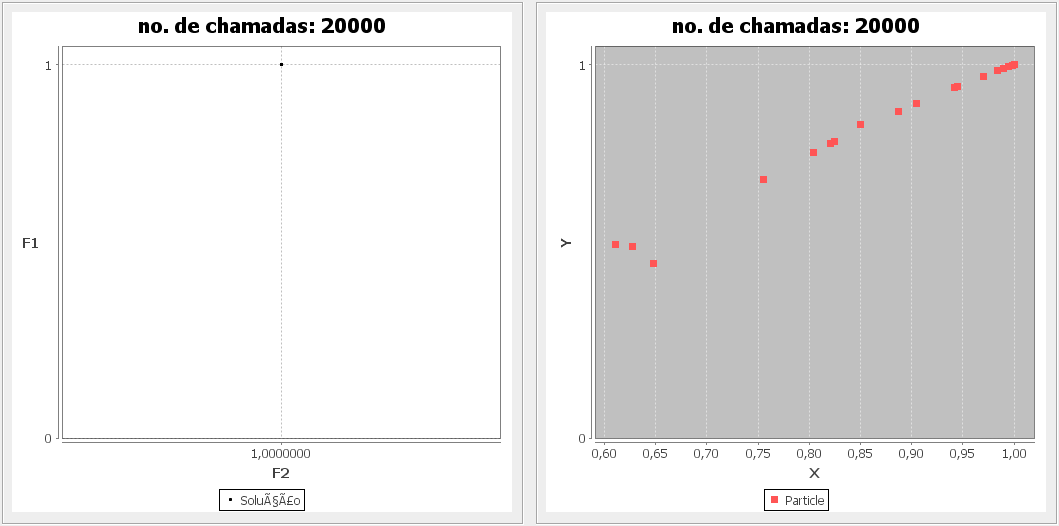
\includegraphics[width=.6\textwidth]{img/result_mopso-cdr_20000_risk.png}
	\caption{Gr\'afico para itera\c{c}\~ao 20000}
	\label{fig:result1}
\end{figure}

A Figura \ref{fig:result2} apresenta so gr\'aficos na itera\c{c}\~ao 20000.
\begin{figure}[H]
	\centering
	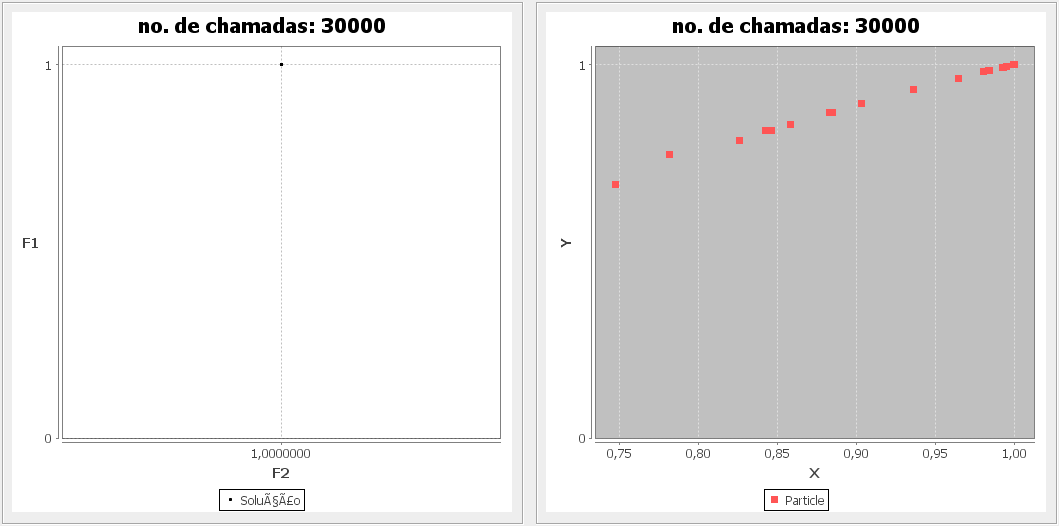
\includegraphics[width=.6\textwidth]{img/result_mopso-cdr_30000_risk.png}
	\caption{Gr\'afico para itera\c{c}\~ao 30000}
	\label{fig:result2}
\end{figure}